\documentclass[xcolor=table,dvipsnames]{beamer}

\usepackage{lscape, amsmath, amsfonts, amssymb, setspace, theorem, wrapfig, graphicx, float, multirow, subfig, color, rotating, multicol, datetime, natbib, venndiagram, pstricks, xkeyval, tikz, etoolbox, verbatim, pgf, tikz, pgfplots, mathrsfs}

\usepackage{listings}
\usepackage{xcolor}
\usetikzlibrary{arrows}

\definecolor{codegreen}{rgb}{0,0.6,0}
\definecolor{codegreengray}{rgb}{0,0.4,0}
\definecolor{codegray}{rgb}{0.5,0.5,0.5}
\definecolor{codeblue}{rgb}{0.00,0,0.82}
\definecolor{backcolour}{rgb}{0.95,0.95,0.92}
\definecolor{jeopardy}{rgb}{.24,.47,.914}

\lstdefinestyle{mystyle}{
    backgroundcolor=\color{backcolour},   
    commentstyle=\color{codegreengray},
    numberstyle=\tiny\color{codegray},
    stringstyle=\color{codegreen},
    basicstyle=\ttfamily\footnotesize,
    breakatwhitespace=false,         
    breaklines=true,                 
    captionpos=b,                    
    keepspaces=true,                 
    numbers=left,                    
    numbersep=5pt,                  
    showspaces=false,                
    showstringspaces=false,
    showtabs=false,                  
    tabsize=2
}
 
\lstset{style=mystyle}

\title{GV300 - Quantitative Political Analysis}
\subtitle{University of Essex - Department of Government}
\date{Week 21 -- 17 February, 2020}				% or you can specify a date, just write it down instead of "\today"
\author{Lorenzo Crippa} 

\usetheme[progressbar=frametitle]{metropolis}
\usecolortheme{seahorse}						% try others: wolverine; crane...


\begin{document}

\begin{frame}[plain]
\begin{center}
\titlepage
\end{center}
\end{frame}

\begin{frame}
\frametitle{Today's session}
Today we will mostly work in two directions: \pause
\begin{enumerate}
\item Some final remarks on the power of a test \pause
\item An exercise on an observational dataset from \cite{card1993}. Try to make a causal claim
\end{enumerate}
\end{frame}

\begin{frame}
\section{Final remarks on the power of a test}
\end{frame}

\begin{frame}
\frametitle{Again on the power of a test}
\begin{itemize}
\item LABa01: power analysis (see R file)
\item LABa02: discussion on the power of a test, $\alpha$, $\beta$ and $1-\beta$ (see R file)
\end{itemize}
\end{frame}

\begin{frame}
\frametitle{The power of a test}
\begin{center}
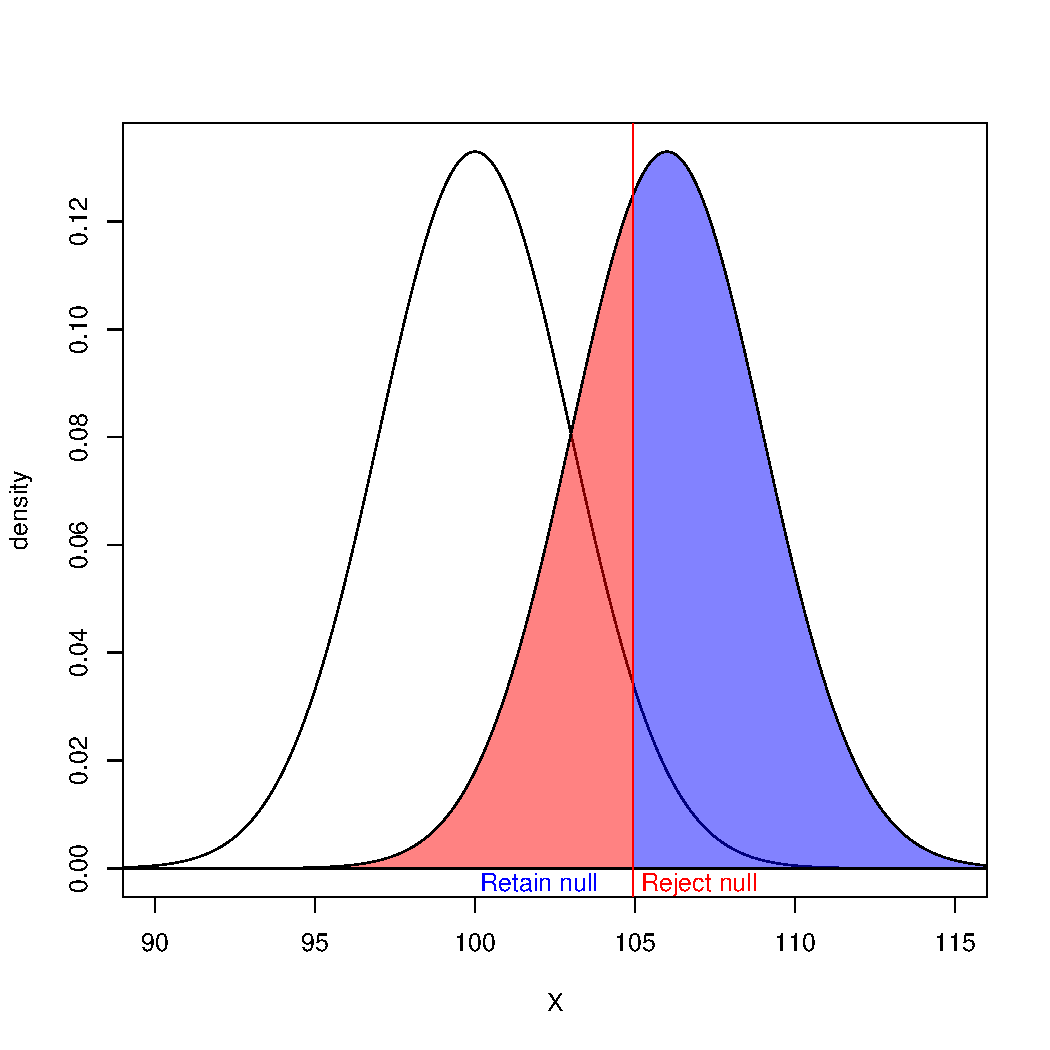
\includegraphics[width = 80mm]{pictures/week_21_power.pdf}
\end{center}
\end{frame}

\begin{frame}
\section{Exercise on observational dataset from Card (1993)}
\end{frame}

\begin{frame}[fragile]
\frametitle{R and Stata session}
Today we are working on the replication data of an article by \cite{card1993}.
You can work alone or in groups of 2. \pause
\begin{enumerate}
\item Download the dataset \texttt{Card\textunderscore data.dta} from Moodle. \pause
\item Open the dataset, look at the variables you have and try to understand what they measure \pause
\item Think about what research question you could answer by using these data. Find a causal claim you can test with them
\end{enumerate}
\end{frame}

\frame{
\frametitle{Card's (1993) research question}
We have a dataset on 3010 subjects, identified by an \texttt{id} variable. \pause We have information on their socio-economic conditions, their education and demographics. \pause

The research question from the author is: \pause

\centering 
\textcolor{red}{Do years of schooling affect wage?}
}


\frame{
\frametitle{Causality and problems}
Think about the causal claim you hypothesize. \pause
\begin{enumerate}
\item Draw a causal diagram representing it \pause
\item What problems could you encounter in estimating the effect? \pause
\item How can you represent these problems?
\end{enumerate}
}

\frame{
\frametitle{Threats to causality}
\begin{tikzpicture}[line cap=round,line join=round,>=triangle 45,x=1cm,y=1cm]
\clip(-0.5,-50) rectangle (28.88,4);
\draw [->,line width=0.6pt, color = NavyBlue] (3,0) -- (6.9,0);
\draw [->,line width=0.6pt] (5,2) -- (3.1,0.1);
\draw [->,line width=0.6pt] (5,2) -- (6.9,0.1);
\draw [->,line width=0.6pt, color = Red] (5,-2) -- (3.1,-0.1);
\draw [->,line width=0.6pt, color = Red] (5,-2) -- (6.9,-0.1);
\begin{scriptsize}
\draw [fill=black, color = NavyBlue] (3,0) circle (1.5pt);
\draw[color=black] (2.5,0.33) node {$Education$};
\draw [fill=black] (7,0) circle (1.5pt);
\draw[color=black] (7.4,0.10) node {$Wage$};
\draw [fill=black] (5,2) circle (1.5pt);
\draw[color=black] (5.16,2.31) node {$Observables$};
\draw [fill=black, color = Red] (5,-2) circle (1.5pt);
\draw[color=black] (5,-2.3) node {$Unobservables$};
\end{scriptsize}
\end{tikzpicture}
}

\frame{
\frametitle{From problems to solutions}
Think about what ways you could solve these problems. \pause
\begin{enumerate}
\item What ideal experiment would let you estimate the effect without bias? \pause Why? \pause
\item What solutions do we have, with observational data, to replicate the conditions of an experiment and \textbf{identify} the causal effect? \pause
	\begin{itemize}
	\item Instrumental variable \pause
	\item Regression discontinuity \pause
	\item Difference-in-differences \pause
	\end{itemize}
\item What \textbf{identification strategy} can you adopt, with these observational data? \pause
\item What do you need to implement it? 
\end{enumerate}
}

\frame{
\frametitle{Solutions}
\begin{enumerate}
\item Controlling for observable does not eliminate the bias \pause $\rightarrow$ unobservable are still out there! \pause
\item In an ideal experiment we would manipulate the years of schooling and randomly assign them to respondents. \pause This way we would eliminate the effect of unobservable confounders on both education and wage \pause
\item Given these observational data, we'd probably need to \textbf{instrument} our independent variable of interest (education) \pause
\item We need a variable that is affecting education but exogenous to our problem (does not impact wage other than through education)\pause $\rightarrow$ exclusion restriction \pause
\end{enumerate}

\textcolor{red}{What instruments could we use in general? Which variable in this dataset?}
}


\frame{
\frametitle{Solution: Instrumental variable!}
\begin{tikzpicture}[line cap=round,line join=round,>=triangle 45,x=1cm,y=1cm]
\clip(-1,-50) rectangle (28.88,4);
\draw [->,line width=0.6pt, color = ForestGreen ] (0,0) -- (2.9,0);
\draw [->,line width=0.6pt, color = NavyBlue] (3,0) -- (6.9,0);
\draw [->,line width=0.6pt] (5,2) -- (3.1,0.1);
\draw [->,line width=0.6pt] (5,2) -- (6.9,0.1);
\draw [->,line width=0.6pt, color = Red] (5,-2) -- (3.1,-0.1);
\draw [->,line width=0.6pt, color = Red] (5,-2) -- (6.9,-0.1);
\begin{scriptsize}
\draw [fill=black, color = ForestGreen] (0,0) circle (1.5pt);
\draw[color=black] (0.22,0.32) node {$Instrument$};
\draw [fill=black, color = NavyBlue] (3,0) circle (1.5pt);
\draw[color=black] (2.5,0.33) node {$Education$};
\draw [fill=black] (7,0) circle (1.5pt);
\draw[color=black] (7.4,0.10) node {$Wage$};
\draw [fill=black] (5,2) circle (1.5pt);
\draw[color=black] (5.16,2.31) node {$Observables$};
\draw [fill=black, color = Red] (5,-2) circle (1.5pt);
\draw[color=black] (5,-2.3) node {$Unobservables$};
\end{scriptsize}
\end{tikzpicture}
}

\frame{
\frametitle{Conduct your analysis entirely}
Now, based on: \pause
\begin{enumerate}
\item Your research question \pause
\item The problem you have for causal inference \pause
\item The identification strategy you have chosen
\end{enumerate}

Conduct the analysis \textbf{entirely}: \pause
\begin{enumerate}
\item Perform a descriptive statistical analysis of the variables of interest \pause You can use all sort of plots (univariate but also bivariate or multivariate), summary statistics, etc. \pause
\item Write down the equation(s) of your research design \pause
\item Estimate the model using your preferred statistical software \pause
\item Interpret the results and present them to the class \pause
\item Do you buy these results? What do you think of the identification strategy?
\end{enumerate}
}

\frame{
\frametitle{Descriptive statistics}
\begin{center}
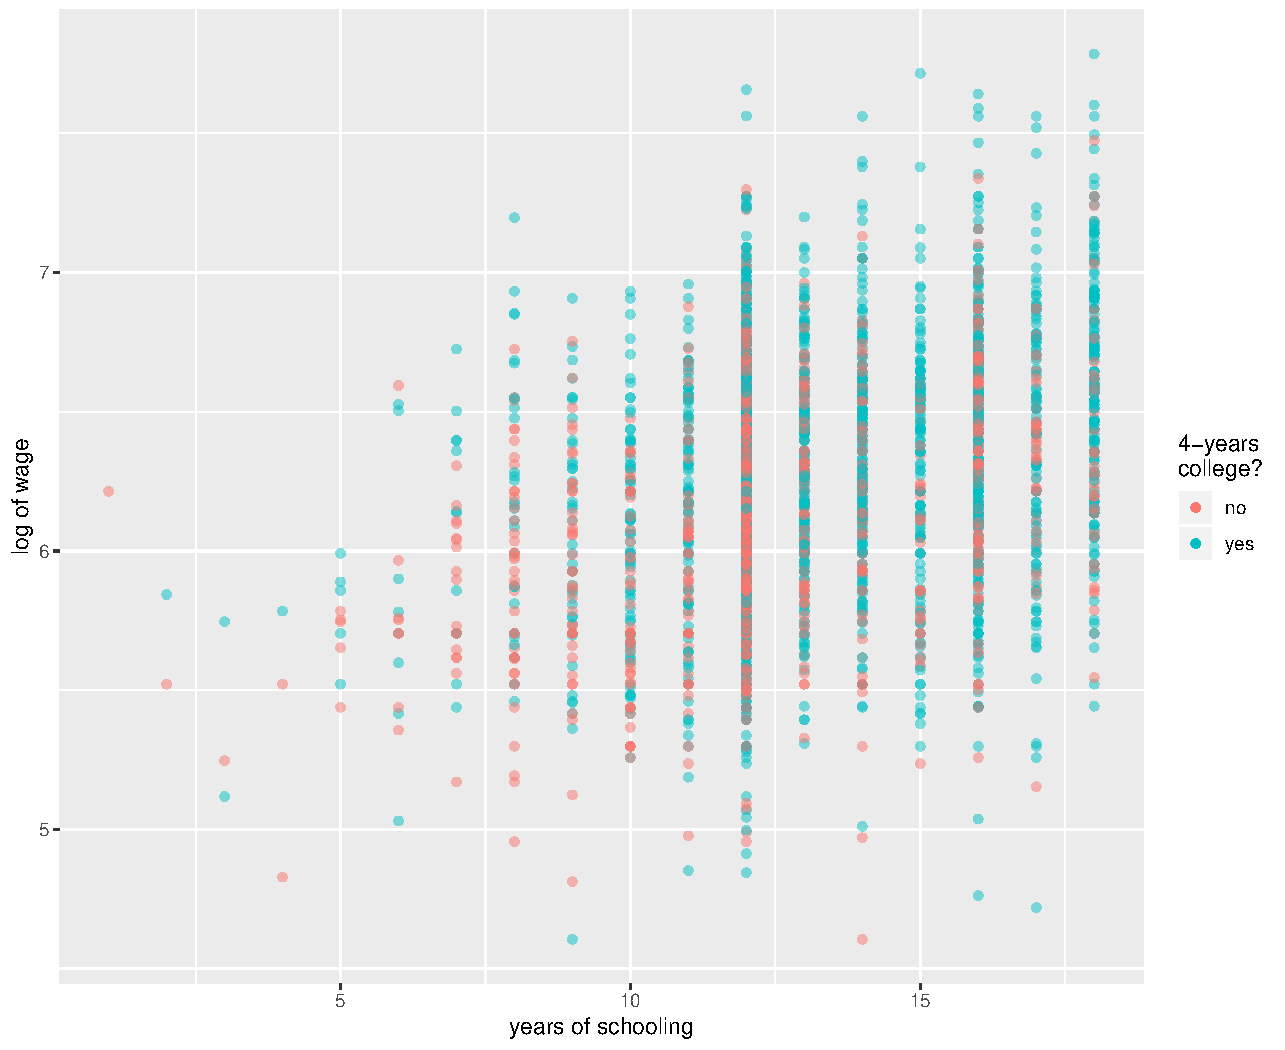
\includegraphics[width = 90mm]{pictures/week_21_scatterplot.pdf}
\end{center}
}

\frame{
\frametitle{Analysis}
The author estimates the causal effect of $education_i$ on $log(wage_i)$ with a two-stage least squares (2SLS) procedure: \pause
$$\widehat{education_i}= \hat{\gamma} + \hat{\delta} college_i + \mathbf{X'_i} \hat{\mathbf{\eta}}$$ \pause
$$log(wage_i) = \hat{\alpha} + \hat{\beta} \widehat{education_i} + \mathbf{X'_i}\hat{\mathbf{\theta}} + u_i$$
}

\frame{
\frametitle{Results}
\begin{table}[!htbp] \centering 
\resizebox{45mm}{40mm}{
\begin{tabular}{l c c }
\hline
 & Model 1 & Model 2 \\
\hline
(Intercept) & $5.06^{***}$  & $4.16^{***}$  \\
            & $(0.07)$      & $(0.84)$      \\
educ        & $0.07^{***}$  & $0.12^{**}$   \\
            & $(0.00)$      & $(0.05)$      \\
exper       & $0.03^{***}$  & $0.06^{***}$  \\
            & $(0.00)$      & $(0.02)$      \\
black1      & $-0.17^{***}$ & $-0.12^{**}$  \\
            & $(0.02)$      & $(0.05)$      \\
south1      & $-0.13^{***}$ & $-0.11^{***}$ \\
            & $(0.02)$      & $(0.02)$      \\
married     & $-0.04^{***}$ & $-0.03^{***}$ \\
            & $(0.00)$      & $(0.01)$      \\
smsa1       & $0.18^{***}$  & $0.15^{***}$  \\
            & $(0.02)$      & $(0.03)$      \\
\hline
R$^2$       & 0.31          & 0.25          \\
Adj. R$^2$  & 0.30          & 0.25          \\
Num. obs.   & 3003          & 3003          \\
\hline
\multicolumn{3}{l}{\scriptsize{$^{***}p<0.01$, $^{**}p<0.05$, $^*p<0.1$}}
\end{tabular}
}
\end{table} 
}

\frame{
\frametitle{Problems}
Are the two requirements for an IV met in this example? \pause 
\begin{enumerate}
\item Strong instrument \pause
\item Exclusion restriction
\end{enumerate}
}

\frame{
\frametitle{Strong instrument?}
\begin{center}
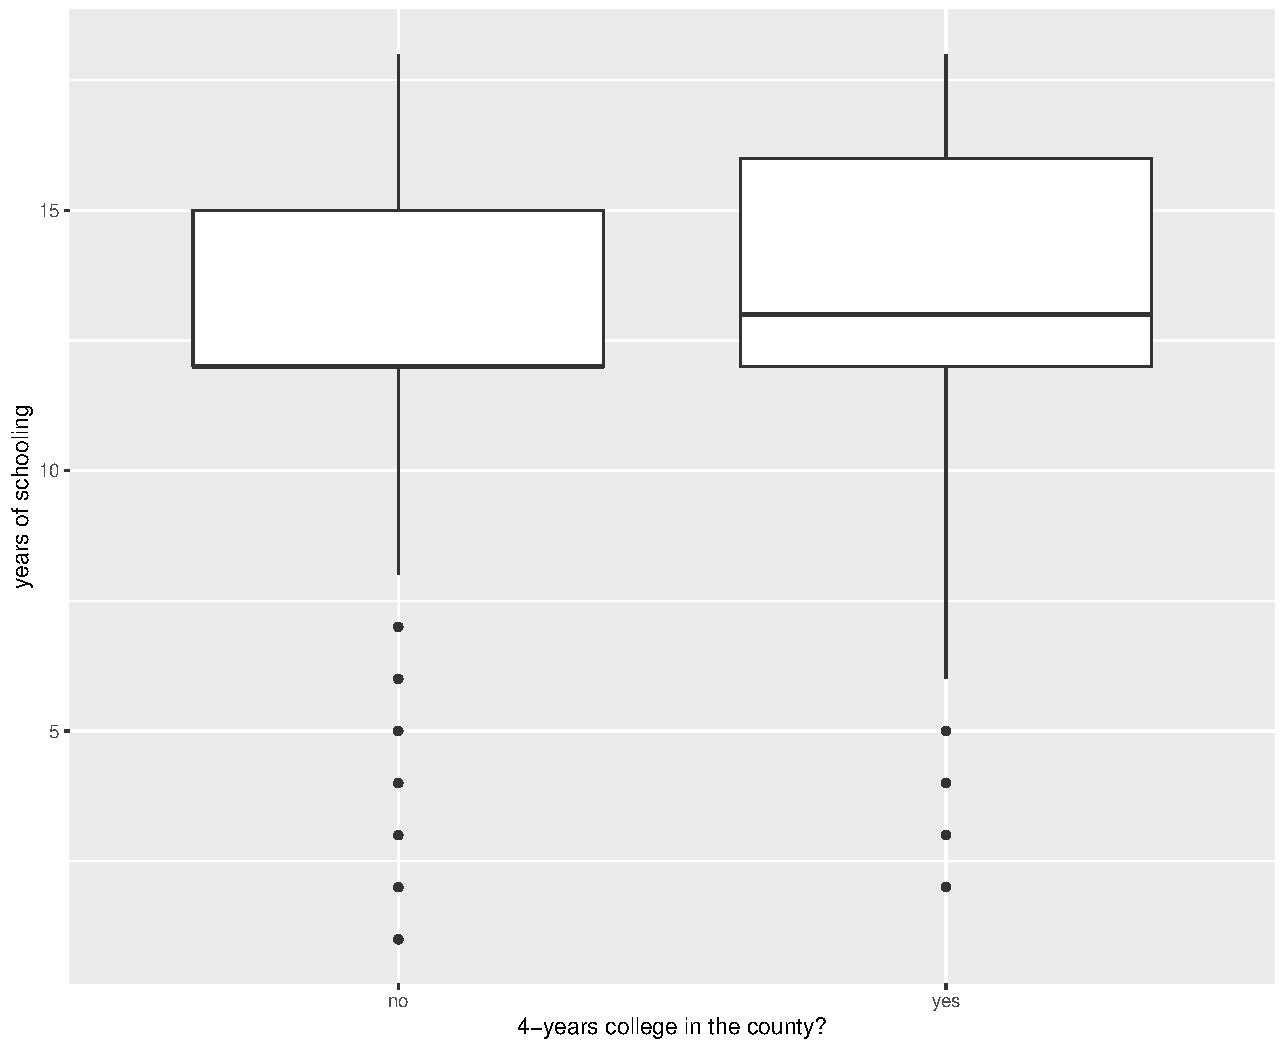
\includegraphics[width = 70mm]{pictures/week_21_boxplot2.pdf}
\end{center}

Does $college_i$ affect years of schooling? \pause Maybe after controlling for observables. \pause

What about the exclusion restriction?
}

\frame{
\frametitle{Exclusion restriction}
Are we sure this never happens? \pause

\begin{tikzpicture}[line cap=round,line join=round,>=triangle 45,x=1cm,y=1cm]
\clip(-1,-4) rectangle (8,3);
\draw [->,line width=0.6pt, color = ForestGreen ] (0,0) -- (2.9,0);
\draw [->,line width=0.6pt, color = Red ] (0,0) -- (4.8,-1.9);
\draw [->,line width=0.6pt, color = NavyBlue] (3,0) -- (6.9,0);
\draw [->,line width=0.6pt] (5,2) -- (3.1,0.1);
\draw [->,line width=0.6pt] (5,2) -- (6.9,0.1);
\draw [->,line width=0.6pt, color = Red] (5,-2) -- (3.1,-0.1);
\draw [->,line width=0.6pt, color = Red] (5,-2) -- (6.9,-0.1);
\begin{scriptsize}
\draw [fill=black, color = ForestGreen] (0,0) circle (1.5pt);
\draw[color=black] (0.22,0.32) node {$4-years college$};
\draw [fill=black, color = NavyBlue] (3,0) circle (1.5pt);
\draw[color=black] (2.5,0.33) node {$Education$};
\draw [fill=black] (7,0) circle (1.5pt);
\draw[color=black] (7.4,0.10) node {$Wage$};
\draw [fill=black] (5,2) circle (1.5pt);
\draw[color=black] (5.16,2.31) node {$Observables$};
\draw [fill=black, color = Red] (5,-2) circle (1.5pt);
\draw[color=black] (5,-2.3) node {$Unobservables$};
\end{scriptsize}
\end{tikzpicture}
}

\frame{
\frametitle{Exclusion restriction}
What do you think about it? Can you think of any variable passing by which the presence of 4-years college affects wage? \pause 

Examples: \pause
\begin{itemize}
\item Social capital ($\neq education$!) \pause
\item Income of a county \pause
\item Possibilities of networking \pause
\end{itemize}

What could a good instrument be, instead?
}

\frame{
\frametitle{Conclusion}
\begin{center}
All clear? More questions? \\
Thanks and see you next week!
\end{center}
}

\begin{frame}
\bibliographystyle{apalike}
\bibliography{week_21}
\end{frame}

\end{document}